%
%
% %%%%%%%%%%%%%%%%%%%%%%%%%%%%%%%%%%%%%%%%%%%%%%%%%%%%%%%%%%%%%%%%%%%%%%
% %%%%%%%%%%%%%%%% Deep Learning with label noise
% %%%%%%%%%%%%%%%%%%%%%%%%%%%%%%%%%%%%%%%%%%%%%%%%%%%%%%%%%%%%%%%%%%%%%%
%
% \section{Label noises}
%
% %%%%%%%% To clarify inputs independence and spatial independence of noises
%
% Label noises can be categoried into three statistical models, noisy complete at random (NCAR), noisy at random (NAR) and noisy not at random (NNAR), based on whether label noises depends on classes and distribution of inputs. (Figure \ref{fig:noises})
% For noisy completely at random models, the occurrence of an error $E$ is independent of neither the true class $Y$ nor the input $X$.
% The noisy at random model is similar to the noisy completely at random model except that the label noise is asymmetric, meaning it depends on classes.
% The noisy at random model model can be interpreted in terms of a transition (or confusion) matrix for $K$ classes:
% \[
% \gamma =
% \begin{bmatrix}
%     P(Y^{\ast}=1\vert Y=1)   & \dots  & P(Y^{\ast}=K\vert Y=1) \\
%     \vdots                   & \ddots & \vdots \\
%     P(Y^{\ast}=1\vert Y=K) & \dots  & P(Y^{\ast}=K\vert Y=K)
% \end{bmatrix}
% \]
% where $Y^{\ast}$ is a random variable for observed label and $Y$ true label.
% The noisy not at random, on the other hand, represents that the label noise depends on both class and example.
%
% \begin{figure}[t]
% \begin{center}
% % \fbox{\rule{0pt}{2in} \rule{0.9\linewidth}{0pt}}
%    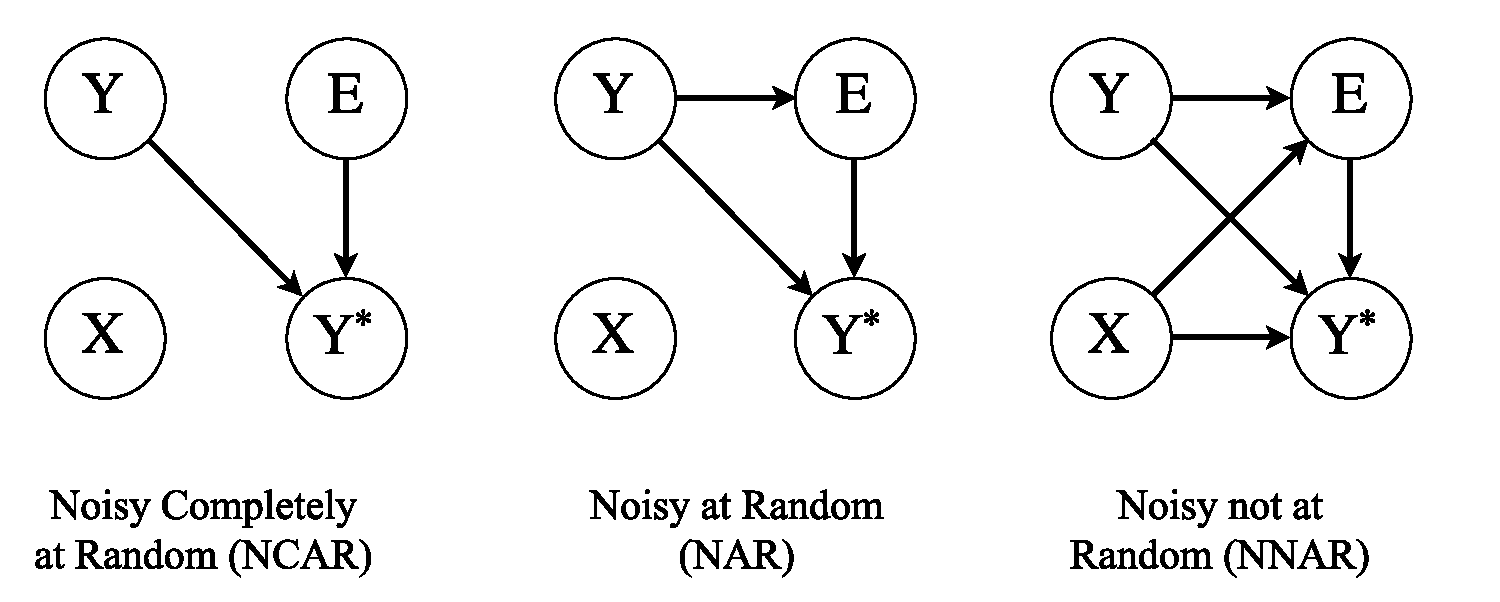
\includegraphics[width=1.05\linewidth]{img/label_noises}
% \end{center}
%    \caption{
%    Graphical models for three types of label noises. \cite{frenay2014classification}
%    The graphical models describe if the probability of the errorness and observed value of a label conditions on the true class and inputs.
%    $X$ is the random variable denotes the inputs;
%    $Y$ is stands for the variable for class;
%    $E$ is a binary variable determining errorness;
%    $Y^{\ast}$ represents a variable for the observed label;
%    }
% \label{fig:noises}
% \end{figure}
%
% In this thesis, we assumed mislabeling of segmentations is noisy at random. {TODO}
